% Dokumentklasse
% --------------
\documentclass[12pt,naustrian,a4widepaper]{scrartcl}   
% article style
%   - 11pt Schriftgroesse
%   - new austrian (neue Rechtschreibung)
%   - Papierformat A4
%   - pdf-hyperlinks

%****************In her all definitions are listed*********************
\usepackage[ngerman]{babel} 					% wegen deutschen Umlauten
\usepackage[utf8]{inputenc}
\usepackage{amsmath}
\usepackage[usenames,dvipsnames]{xcolor}
\usepackage{pdfpages}
\usepackage{lastpage} 							% Required to determine the last page for the footer
%\usepackage{amsmath}
\usepackage{float}
\usepackage{hyperref}
\usepackage{listings}
\usepackage{graphicx}							% Einbinden von Bildern
%\usepackage{multicol} 							% Spalten
%\usepackage{textcomp} 							% spitze klammern
%\usepackage{hyperref}  						% hyperlinks
\usepackage[absolute]{textpos}
\usepackage{xcolor}
\usepackage{tabularx}
\usepackage{tcolorbox}
\usepackage{enumitem}
\usepackage{fancyhdr}   % für Kopf- und Fusszeilen
%*************************************************************************
\pagestyle{fancy} 						% Wird für den Header gebraucht

% Seitenspiegel
% -------------

\typearea{8}	% Festlegung des Seitenspiegels gem. Koma. 4..groß, 9..klein


% Kopfzeile
% ---------
\lhead{{\footnotesize{\docauthor, \doccoauthor}}}   %  (links)
\chead{{\footnotesize{Systemdokumentation - \docproject}}} %  (mitte)
\rhead{{\footnotesize{Seite \thepage}}}      %  (rechts)

% Fusszeile
% ---------
\lfoot{}  % links
\cfoot{}  % mitte 
\rfoot{}  % rechts

% Absatzformatierung
% ------------------
\setlength{\parindent}{0cm}   % Einrückung der 1. Zeile jedes Absatzes
\setlength{\parskip}{10pt}    % Abstand zwischen den Absätzen

\selectlanguage{naustrian}   % oder "american" für engl. Texte

% Titelblatt
% ----------
\newcommand{\hgbtitle}{
\title {\vspace{1cm}
	
\includegraphics[width=8cm]{./Images/FhOOeLogoOkt2009_HSD_Rot_pastell}\\
	\vspace{2cm}
	{\textbf{Systemdokumentation\\Projekt \docproject}}\\
	\vspace{5mm}
	{\small{Version 1.0}}\\
	\vspace{5mm}
}

\author{\small{\docauthor, \doccoauthor}}
\date  {\small{Hagenberg, \today}}
\maketitle
}

%****************** self defined commands ***************************
%include a pseudocode file
%usage: \pseudocode{Title}{path_to_your_file/filename} (relative to Übung root folder)
\newcommand{\pseudocode}[2]{
\begin{itemize}
\item[]\lstinputlisting[caption="#1",label="#1", style=pseudocodeStyle]{../#2}
\end{itemize}
}

% Include Linux terminal output
% Usage: \linuxoutput{Title}{path_to_your_file/filename}
\newcommand{\linuxoutput}[2]{
	\begin{itemize}
		\item[]\lstinputlisting[
		caption="#1",
		label="#1",
		style=linuxStyle
		]{../#2}
	\end{itemize}
}

% include an ARM Assembly source file
% usage: \armasm{path_to_your_file/filename}
%        (relative to Übung root folder)
\newcommand{\armasm}[1]{
	\begin{itemize}
		\item[]\lstinputlisting[
		caption="#1.s",
		label="#1.s",
		style=armasm
		]{../#1.s}
	\end{itemize}
}

% Usage: \bashscript{Title}{path_to_script}
\newcommand{\bashscript}[2]{
	\begin{itemize}
		\item[]\lstinputlisting[caption="#1",label="#1",style=bashStyle]{../#2}
	\end{itemize}
}

%include a .cpp source file
%usage: \cpp{path_to_your_file/filename}(relative to Übung root folder)
\newcommand{\cpp}[1]{
\begin{itemize}
\item[]\lstinputlisting[caption="#1.cpp",label="#1.cpp", style=customcpp]{../#1.cpp}
\end{itemize}
}

%include a .c source file
%usage: \cfile{path_to_your_file/filename}(relative to Übung root folder)
\newcommand{\cfile}[1]{
	\begin{itemize}
		\item[]\lstinputlisting[caption="#1.c",label="#1.c", style=customcpp]{../#1.c}
	\end{itemize}
}

%include a .h source file
%usage: \h{path_to_your_file/filename} (relative to Übung root folder)
\newcommand{\h}[1]{
\begin{itemize}
\item[]\lstinputlisting[caption="#1.h",label="#1.h", style=customcpp]{../#1.h}
\end{itemize}
}

%include a module (.cpp and .h)
%usage: \cppmodule{path_to_your_file/filename} (relative to Übung root folder)
\newcommand{\cppmodule}[1]{
\begin{itemize}
\item[]\lstinputlisting[caption=#1.h,label=#1.h, style=customcpp]{../#1.h}
\item[]\lstinputlisting[caption=#1.cpp,label=#1.cpp, style=customcpp]{../#1.cpp}
\end{itemize}
}

%include a code snippet
%usage: \snippet{path_to_your_file/filename}{startline}{endline} (relative to Übung root folder)
\newcommand{\snippet}[3]{
\begin{itemize}
\item[]\lstinputlisting[caption=#1.cpp,label=#1.cpp, style=customcpp, firstline=#2,lastline=#3]{../#1.cpp}
\end{itemize}
}

%include a test-output file 
%usage: \testoutput{path_to_your_file/filename} (relative to Übung root folder)
\newcommand{\testoutput}[1]{
\begin{itemize}
\item[]\lstinputlisting[caption=#1]{../#1.txt}
\end{itemize}
}

%include a figure 
%usage: \fig{path_to_your_file/filename}{width}{caption text} (relative to Übung root folder)
%width between 0.0 - 1.0 -> correspond with textwidth
\newcommand{\fig}[3]{
\begin{figure}[H]
\centering
\includegraphics[width=#2\textwidth]{../#1}
\caption{#3}
\label{fig:fig1}
\end{figure}
}

%include a flowchart
%usage: \flow{path_to_your_file/filename} (relative to Übung root folder)
\newcommand{\flow}[3]{
\begin{figure}[H]
\centering
\includegraphics[width=0.5\textwidth]{../#1.png}
\caption{Flussdiagramm #1}
\label{fig:fig1}
\end{figure}
}


\lstset{
   literate      = 
      {á}{{\'a}}1  {é}{{\'e}}1  {í}{{\'i}}1 {ó}{{\'o}}1  {ú}{{\'u}}1
      {Á}{{\'A}}1  {É}{{\'E}}1  {Í}{{\'I}}1 {Ó}{{\'O}}1  {Ú}{{\'U}}1
      {à}{{\`a}}1  {è}{{\`e}}1  {ì}{{\`i}}1 {ò}{{\`o}}1  {ù}{{\`u}}1
      {À}{{\`A}}1  {È}{{\`E}}1  {Ì}{{\`I}}1 {Ò}{{\`O}}1  {Ù}{{\`U}}1
      {ä}{{\"a}}1  {ë}{{\"e}}1  {ï}{{\"i}}1 {ö}{{\"o}}1  {ü}{{\"u}}1
      {Ä}{{\"A}}1  {Ë}{{\"E}}1  {Ï}{{\"I}}1 {Ö}{{\"O}}1  {Ü}{{\"U}}1
      {â}{{\^a}}1  {ê}{{\^e}}1  {î}{{\^i}}1 {ô}{{\^o}}1  {û}{{\^u}}1
      {Â}{{\^A}}1  {Ê}{{\^E}}1  {Î}{{\^I}}1 {Ô}{{\^O}}1  {Û}{{\^U}}1
      {œ}{{\oe}}1  {Œ}{{\OE}}1  {æ}{{\ae}}1 {Æ}{{\AE}}1  {ß}{{\ss}}1
      {ẞ}{{\SS}}1  {ç}{{\c{c}}}1 {Ç}{{\c{C}}}1 {ø}{{\o}}1  {Ø}{{\O}}1
      {å}{{\aa}}1  {Å}{{\AA}}1  {ã}{{\~a}}1  {õ}{{\~o}}1 {Ã}{{\~A}}1
      {Õ}{{\~O}}1  {ñ}{{\~n}}1  {Ñ}{{\~N}}1  {¿}{{?`}}1  {¡}{{!`}}1
      {„}{\quotedblbase}1 {“}{\textquotedblleft}1 {–}{$-$}1
      {°}{{\textdegree}}1 {º}{{\textordmasculine}}1 {ª}{{\textordfeminine}}1
      {£}{{\pounds}}1  {©}{{\copyright}}1  {®}{{\textregistered}}1
      {«}{{\guillemotleft}}1  {»}{{\guillemotright}}1  {Ð}{{\DH}}1  {ð}{{\dh}}1
      {Ý}{{\'Y}}1    {ý}{{\'y}}1    {Þ}{{\TH}}1    {þ}{{\th}}1    {Ă}{{\u{A}}}1
      {ă}{{\u{a}}}1  {Ą}{{\k{A}}}1  {ą}{{\k{a}}}1  {Ć}{{\'C}}1    {ć}{{\'c}}1
      {Č}{{\v{C}}}1  {č}{{\v{c}}}1  {Ď}{{\v{D}}}1  {ď}{{\v{d}}}1  {Đ}{{\DJ}}1
      {đ}{{\dj}}1    {Ė}{{\.{E}}}1  {ė}{{\.{e}}}1  {Ę}{{\k{E}}}1  {ę}{{\k{e}}}1
      {Ě}{{\v{E}}}1  {ě}{{\v{e}}}1  {Ğ}{{\u{G}}}1  {ğ}{{\u{g}}}1  {Ĩ}{{\~I}}1
      {ĩ}{{\~\i}}1   {Į}{{\k{I}}}1  {į}{{\k{i}}}1  {İ}{{\.{I}}}1  {ı}{{\i}}1
      {Ĺ}{{\'L}}1    {ĺ}{{\'l}}1    {Ľ}{{\v{L}}}1  {ľ}{{\v{l}}}1  {Ł}{{\L{}}}1
      {ł}{{\l{}}}1   {Ń}{{\'N}}1    {ń}{{\'n}}1    {Ň}{{\v{N}}}1  {ň}{{\v{n}}}1
      {Ő}{{\H{O}}}1  {ő}{{\H{o}}}1  {Ŕ}{{\'{R}}}1  {ŕ}{{\'{r}}}1  {Ř}{{\v{R}}}1
      {ř}{{\v{r}}}1  {Ś}{{\'S}}1    {ś}{{\'s}}1    {Ş}{{\c{S}}}1  {ş}{{\c{s}}}1
      {Š}{{\v{S}}}1  {š}{{\v{s}}}1  {Ť}{{\v{T}}}1  {ť}{{\v{t}}}1  {Ũ}{{\~U}}1
      {ũ}{{\~u}}1    {Ū}{{\={U}}}1  {ū}{{\={u}}}1  {Ů}{{\r{U}}}1  {ů}{{\r{u}}}1
      {Ű}{{\H{U}}}1  {ű}{{\H{u}}}1  {Ų}{{\k{U}}}1  {ų}{{\k{u}}}1  {Ź}{{\'Z}}1
      {ź}{{\'z}}1    {Ż}{{\.Z}}1    {ż}{{\.z}}1    {Ž}{{\v{Z}}}1  {ž}{{\v{z}}}1
      {¢}{{$\not\subset$}}1 {§}{{\S}}1 {¥}{{\textyen}}1   ,
   inputencoding=ansinew,
   extendedchars=true,
   basicstyle=\scriptsize\ttfamily,
   numberstyle=\scriptsize,
   breaklines=true,
   tabsize=4,
   numbersep=5pt
}

\lstdefinestyle{customcpp}{
   language=C++,
   frame=single,
   %backgroundcolor=\color{mygray},
   numbers=left,
   keywordstyle=\color{blue}\bfseries,
   stringstyle=\color{BrickRed}\ttfamily,
   commentstyle=\color{OliveGreen}\ttfamily,
   showspaces=false,
   showstringspaces=false,
   showtabs=false,
   xleftmargin=5px,    
}

\usepackage[T1]{fontenc}
\usepackage[utf8]{inputenc}
\usepackage[dvipsnames]{xcolor}
\usepackage{listings}
\usepackage{lmodern}

% --------------------------------------------------------------------------
% ARM Assembly language definition
% --------------------------------------------------------------------------
\lstdefinelanguage{ARMASM}{
	morekeywords=[1]{
		AREA,ALIGN,ALIGNR,ATTR,EXPORT,IMPORT,PROC,ENDP,END,
		PRESERVE8,THUMB,CODE,DATA,READONLY,READWRITE,NOINIT,
		DCD,DW,DCW,DCB,SPACE,EQU
	},
	morekeywords=[2]{
		LDR,STR,LDM,STM,LDMIA,STMIA,
		PUSH,POP,MOV,MVN,
		ADD,ADC,SUB,SBC,MUL,MLS,MLA,
		AND,ORR,EOR,BIC,
		CMP,CMN,TST,TEQ,
		B,BL,BX,BLX,
		BEQ,BNE,BCS,BHS,BCC,BLO,
		BMI,BPL,BVS,BVC,BHI,BLS,
		BGE,BLT,BGT,BLE
	},
	morekeywords=[3]{
		R0,R1,R2,R3,R4,R5,R6,R7,
		R8,R9,R10,R11,R12,SP,LR,PC,
		APSR,CPSR
	},
	morekeywords=[4]{
		DCD,DW,DCW,DCB,SPACE,EQU
	},
	sensitive=false,
	morecomment=[l]{;},
	morestring=[b]"
}

% --------------------------------------------------------------------------
% ARM Assembly style
% --------------------------------------------------------------------------
\definecolor{armblue}{RGB}{0,70,140}
\definecolor{armgreen}{RGB}{0,120,70}
\definecolor{armred}{RGB}{170,40,40}
\definecolor{armgray}{RGB}{100,100,100}
\definecolor{armpurple}{RGB}{110,50,140}

\lstdefinestyle{armasm}{
	language=ARMASM,
	basicstyle=\ttfamily\small,
	columns=fullflexible,
	keepspaces=true,
	keywordstyle=[1]\color{armblue}\bfseries,
	keywordstyle=[2]\color{armred}\bfseries,
	keywordstyle=[3]\color{armpurple},
	keywordstyle=[4]\color{armgreen}\bfseries,
	commentstyle=\color{armgray}\itshape,
	stringstyle=\color{armgreen},
	numbers=left,
	numberstyle=\tiny\color{armgray},
	numbersep=8pt,
	frame=single,
	rulecolor=\color{black!25},
	framesep=5pt,
	breaklines=true,
	breakatwhitespace=false,
	showstringspaces=false,
	tabsize=8,	
	captionpos=b
}


\lstdefinelanguage{linux}{
	sensitive=true,
	morekeywords={cd,ls,cat,touch,rm,mkdir,rmdir,cp,mv,pwd,echo,grep,find,chmod,chown,tar,clear,exit},
	morestring=[b]"
}

\lstdefinestyle{linuxStyle}{
	language=linux,
	frame=single,
	numbers=none,
	basicstyle=\ttfamily\footnotesize\color{black},
	keywordstyle=\color{Blue}\bfseries,
	stringstyle=\color{BrickRed},
	emph={tlech@DESKTOP,MPJVO86},
	emphstyle=\color{Green}\bfseries,
	showspaces=false,
	showstringspaces=false,
	showtabs=false,
	breaklines=true,
	breakatwhitespace=false,
	xleftmargin=5px,
	literate=
	{_}{{\_}}1
	{ä}{{\"a}}1
	{ö}{{\"o}}1
	{ü}{{\"u}}1
	{Ä}{{\"A}}1
	{Ö}{{\"O}}1
	{Ü}{{\"U}}1
	{ß}{{\ss}}1
}

\lstdefinelanguage{bash}{
	sensitive=true,
	morekeywords={
		if,then,else,elif,fi,
		for,while,until,in,
		do,done,
		case,esac,
		function,
		select,
		time,
		coproc,
		return,
		local,
		declare,
		readonly,
		export,
		unset,
		shift,
		getopts,
		source,
		echo,
		printf,
		read,
		cd,
		pwd,
		test,
		true,
		false,
		type,
		command,
		builtin,
		eval,
		exec,
		exit,
		let
	},
	morestring=[b]",
	morestring=[b]',
	morecomment=[l]\#
}

\lstdefinestyle{bashStyle}{
	language=bash,
	frame=single,
	numbers=left,
	numberstyle=\tiny\color{gray},
	basicstyle=\ttfamily\small\color{black},
	keywordstyle=\color{Blue}\bfseries,
	stringstyle=\color{BrickRed},
	commentstyle=\color{OliveGreen},
	showspaces=false,
	showstringspaces=false,
	showtabs=false,
	breaklines=true,
	breakatwhitespace=false,
	keepspaces=true,
	columns=fullflexible,
	xleftmargin=5px
}


\lstdefinelanguage{pseudocode}{
  morekeywords={if, then, else, elseif, case, of, while, do, repeat, until, for, to, by, end, algorithm, const, static, bool, int, char, double, string, real, array, param, local, modulo, halt, return, not, size\_t, and, or, xor},
  sensitive=true,
  morecomment=[l]{//},
  morestring=[b]"
}

% Define a style for pseudocode listings
\lstdefinestyle{pseudocodeStyle}{
  language=pseudocode,
   frame=none,
   numbers=none,
   keywordstyle=\underline,
   stringstyle=\color{BrickRed}\ttfamily,
   commentstyle=\color{OliveGreen}\ttfamily,
   showspaces=false,
   showstringspaces=false,
   showtabs=false,
   xleftmargin=5px,
   literate={!=}{{$\neq$}}1
   			{=}{{$\leftarrow$}}1 
   			{==}{{$==$}}1
   			{<=}{{$\leq$}}1
   			{>=}{{$\geq$}}1
   			{°}{{$\downarrow$}}1 
			{\#}{{$\updownarrow$}}1 
   			{^}{{$\uparrow$}}1 
   			{ö}{{\"o}}1
           	{ä}{{\"a}}1
           	{ü}{{\"u}}1
           	{ß}{{\ss}}1
           	{é}{{\'e}}1
}


% For function descriptions
% ---------- Parameter ----------
\newcommand{\param}[1]{\item #1}

% ---------- Function Command ----------
% #1 function signature
% #2 parameter items (\param{...})
% #3 description
\newcommand{\func}[3]{%
\begin{tcolorbox}[
    colback=white,          % white background for main box
    colframe=black!50,      % subtle border
    colbacktitle=white,     % white background for the title/header
    coltitle=black,         % black text for the title
    boxrule=0.6pt,          % border thickness
    arc=1mm,                % rounded corners
    left=6pt, right=6pt, top=4pt, bottom=4pt,
    fonttitle=\ttfamily\bfseries,
    title={#1}              % function signature in header
]
% Only show parameters if provided
\ifx&#2&%
  % do nothing
\else
\textbf{Parameter}%
\begin{itemize}[topsep=0pt, partopsep=0pt, parsep=0pt, itemsep=0pt, leftmargin=*]
#2
\end{itemize}
\fi

\textbf{Beschreibung} #3

\end{tcolorbox}%
\vspace{2pt} % minimal spacing after box
}

%*************************Dokumenteninfos*******************************
\newcommand{\docproject}{Player-Schnittstelle}			% Projektname
\newcommand{\docsubject}{Software Design Patterns}	% Fach
\newcommand{\docsubjectshort}{SDP3}					% Fach-Kürzl
\newcommand{\docexercise}{Übung 3}					% Übungstitel
\newcommand{\docauthor}{T. Lechner}					% Name
\newcommand{\doccoauthor}{P. Ackermann}				% Name
\newcommand{\docauthornumber}{S2510306017}			% Martrikelnummer
\newcommand{\doccoauthornumber}{S2510306001}		% Martrikelnummer
\newcommand{\docauthoremail}{s2510306017@students.fh-hagenberg.at}
\newcommand{\doccoauthoremail}{s2510306001@students.fh-hagenberg.at}
\newcommand{\docdate}{\date}						% Datum	
\newcommand{\docsemester}{Wintersemester 2026/2027}	% Semester
%%%%%%%%%%%%%%%%%%%%%%%%%%%%%%%%%%%%%%%%%%%%%%%%%%%%%%%%%%%%%

\begin{document}


%%%%%%%%%%%%%%%%%%%%%%%%%%%%%%% Angabe.pdf %%%%%%%%%%%%%%%%%%%%%%%%%%%%%%%
\begin{textblock*}{80mm}(43mm,70mm)
	\docauthor, \doccoauthor
\end{textblock*}
\begin{textblock*}{80mm}(44mm,84mm)
	\docauthornumber, \doccoauthornumber
\end{textblock*}
\begin{textblock*}{40mm}(60mm,99mm)
	1 					% Übungsgruppe
\end{textblock*}
\begin{textblock*}{40mm}(155mm,70mm)
	13					% Stunden
\end{textblock*}

% Inkludieren der Angabe
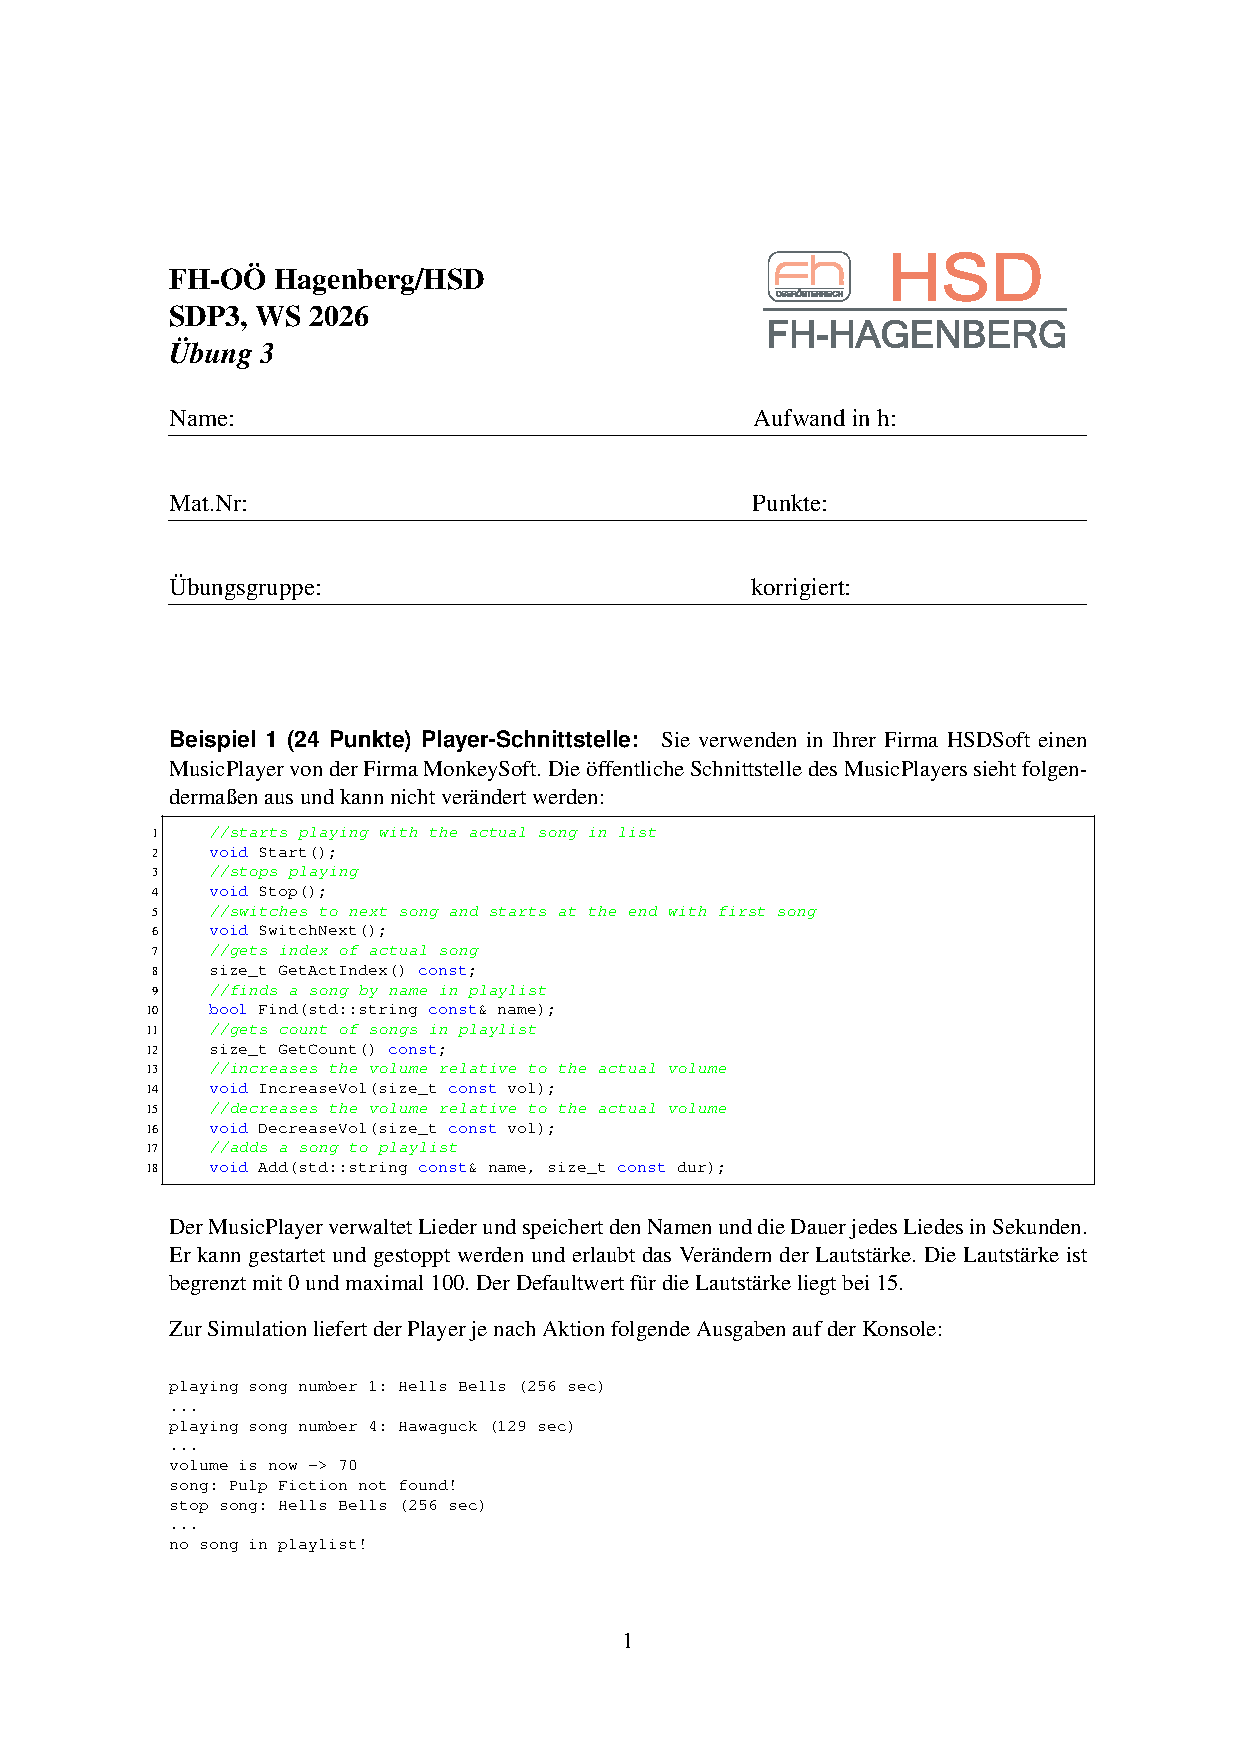
\includepdf[pages=-]{Angabe.pdf}
\newpage
\hgbtitle
\newpage


%%%%%%%%%%%%%%%%%%%%%%%%%%%%%%% Inhaltsverzeichnis %%%%%%%%%%%%%%%%%%%%%%%%

\tableofcontents
\newpage

%%%%%%%%%%%%%%%%%%%%%%%%%%%%%%% Ausarbeitung %%%%%%%%%%%%%%%%%%%%%%%%%%%%%%

\section{Organisatorisches}

\subsection{Team}
\begin{itemize}
	\item \docauthor, Matr.-Nr.: \docauthornumber, E-Mail: \docauthoremail	
	\item \doccoauthor, Matr.-Nr.: \doccoauthornumber, E-Mail: \doccoauthoremail
\end{itemize}

\subsection{Aufteilung der Verantwortlichkeitsbereiche}
\begin{itemize}
	\item \docauthor
	\begin{itemize}
		\item Anforderungsdefinition
		\item Implementierung und Unit-Test:
		\begin{itemize}
			\item Video
			\item Object
			\item IMediaPlayer
			\item VideoFormat
			\item VideoPlayer
			\item VideoPlayerAdapter
		\end{itemize}
	\end{itemize}
	\item \doccoauthor
	\begin{itemize}
		\item Designentscheidungen
		\item Implementierung und Unit-Test:
		\begin{itemize}
			\item Song
			\item MusicPlayer
			\item MusicPlayerAdapter
			\item PlayerClient
		\end{itemize}
	\end{itemize}	
\end{itemize}

\subsection{Aufwand}

\begin{itemize}
	\item \docauthor: geschätzt 6 Ph / tatsächlich 7 Ph
	\item \doccoauthor: geschätzt 6 Ph / tatsächlich 6 Ph
\end{itemize}

\section{Anforderungsdefinition (Systemspezifikation)}
\subsection{MonkeySoft}
Es soll ein Musik Player implementiert werden. Dieser kann mehrere Songs, bestehend aus Titel und Dauer in Sekunden in seiner Playlist speichern.\\
Die Songs können abgespielt und das Abspielen wieder gestoppt werden. Es gibt auch die Möglichkeit, auf den nächsten Song zu wechseln, wenn alle Songs durch sind, wird wieder von vorne angefangen.\\
Der Musik Player verfügt über eine Lautstärke (0 bis 100, standardmäßig 15), die erhöht und verringert werden kann.\\
Neue Songs können hinzugefügt werden und es kann nach einem bestimmten Titel gesucht werden.\\
Die Anzahl der Songs in der Playlist und der Index des aktuell ausgewählten Songs kann ermittelt werden.

\subsection{DonkeySoft}
Es soll ein Video Player implementiert werden. Dieser kann mehrere Videos, bestehend aus Titel, Video-Format (AVI, MKV oder WMV) und Dauer in Minuten in seiner Playlist speichern.\\
Die Videos können abgespielt und das Abspielen wieder gestoppt werden. Es gibt auch die Möglichkeit, auf das nächste Video zu wechseln und wieder auf den Anfang zurückzuspringen.\\
Der Musik Player verfügt über eine Lautstärke (0 bis 50, standardmäßig 8), die erhöht und verringert werden kann.\\
Neue Videos können hinzugefügt werden.\\
Der Titel und Index des aktuell ausgewählten Videos kann auch ermittelt werden.

\subsection{HSDSoft}
Es soll für einen Klienten die oben genannten Player in einem einheitlichen Format mit einer gemeinsamen Schnittstelle bereitgestellt werden. Mit dieser Schnittstelle können beide Player gestartet und gestoppt werden. Es kann zwischen Liedern/Videos vor und zurück gewechselt werden. Wird über den Anfang hinaus zurückgewechselt, springt der Player wieder zum Ende. Wird das Ende überschritten, so fängt er wieder von vorne an. Die Lautstärke kann auch immer um 1 erhöht/verringert werden, bis die minimale/maximale Lautstärke erreicht ist. Es kann auch ein ganz bestimmter Titel (sofern dieser existiert) basierend auf dem Namen ausgewählt werden.\\

Das Hinzufügen neuer Medien ist über die Schnittstelle nicht möglich, sondern nur das Bedienen bereits ausgestatteter Player.\\


\section{Systementwurf}

\subsection{Klassendiagramm}
\fig{Systemdoku/Images/MediaPlayer.png}{1.2}{Klassendiagramm \docproject}

\subsection{Designentscheidungen}
Um bei weiterer Ableitung der verwendeten Klassen bereits einen virtuellen Destruktor bereitzustellen, werden alle Klassen mit Ausnahme von Interfaces von einer gemeinsamen Object-Klasse mit virtuellem Destruktor abgeleitet.\\

Da die Klasse Client eine einheitliche Schnittstelle von sowohl dem MusicPlayer als auch dem MediaPlayer benötigt, wird hier das Softwarepattern des Adapters angewandt. Hierbei werden für beide Klassen jeweils eine Adapter Klasse bereitgestellt, welche die gemeinsamen Funktionalitäten dem Client bereitstellen sollen. Diese Adapter erben von einem gemeinsamen Interface, damit auch später weitere Adapter für andere Klassen mit ähnlichen Funktionalitäten hinzugefügt werden können.
Die Adapter Klassen müssen jeweils Objekte ihrer Klassen, die sie adaptieren aggregieren. So können auf deren Member über ihre Getter zugegriffen werden und auch andere bereitgestellte Methoden verwendet werden.\\

\textbf{MusicPlayer:}\\
Um den Zustand der Lautstärke, der über die vorgegebenen Methoden geändert werden soll zu speichern, wird ein Member verwendet. Ebenso wird ein Vector aus „Songs“ zur praktikablen Speicherung der Lieder verwendet. Die Klasse Songs wiederum beinhaltet Member zur Speicherung von Titel und Dauer. Es werden Getter-Methoden zum Lesen zu Verfügung gestellt. Das nachträgliche Ändern soll nur für den Namen möglich sein, da die Länge eines Songs als konstant angenommen wird.\\

\textbf{VideoPlayer:}\\
Ebenso wie im MusicPlayer muss auch hier der Zustand der Lautstärke und die einzelnen Videos gespeichert werden können. Für ein Video werden Member für Namen und Länge, aber auch für das Dateiformat benötigt. Die Werte für dieses Dateiformat, werden über ein Enum „Videoformat“ definiert.\\

Hinweis: Die Adapter für den MusicPlayer und den VideoPlayer werden wie in der Angabe gefordert über die Klasse PlayerClient ausführlich getestet. Da einige Methoden der Klassen, die die Adapter aggregieren von den Adaptermethoden nicht verwendet werden, müssen diese Klassen (MusicPlayer, Song, VideoPlayer, Video) eigenen Unit-Tests unterzogen werden.\\

\section{Dokumentation der Komponenten (Klassen)}

Die HTML-Startdatei befindet sich im Verzeichnis \href{run:./../doxy/html/index.html}{./../doxy/html/index.html}

\section{Testprotokollierung}

Die Tests wurden mittels Google Test Suite direkt in Visual Studio durchgeführt.
\testoutput{Systemdoku/Tests}

\section{Quellcode}
\subsubsection{Object}
\h{Beispiel01/Object}

\subsection{MonkeySoft}
\subsubsection{Song}
\cppmodule{Beispiel01/Song}
\subsubsection{MusicPlayer}
\cppmodule{Beispiel01/MusicPlayer}


\subsection{DonkeySoft}
\subsubsection{VideoFormat}
\cppmodule{Beispiel01/VideoFormat}
\subsubsection{Video}
\cppmodule{Beispiel01/Video}
\subsubsection{VideoPlayer}
\cppmodule{Beispiel01/VideoPlayer}


\subsection{HSDSoft}
\subsubsection{IMediaPlayer}
\h{Beispiel01/IMediaPlayer}
\subsubsection{MusicPlayerAdapter}
\cppmodule{Beispiel01/MusicPlayerAdapter}
\subsubsection{VideoPlayerAdapter}
\cppmodule{Beispiel01/VideoPlayerAdapter}
\subsubsection{PlayerClient}
\cppmodule{Beispiel01/PlayerClient}

\subsection{Testtreiber}
\cpp{Beispiel01/Test}

\end{document}
%%%%%%%%%%%%%%%%%%%%%%%%%%%%%%%%%%%%%%%%%%%%%%%%%%%%%%%%%%%%%%%%%%%%%%%%%%%